\chap{LED Animations}

\section{Exercise and Report}
\subsection{Exercise 1}
From the simulation on Proteus, one more LED is connected to pin \textbf{PA6} of the STM32 (negative pin of the LED is connected to PA6). The component suggested in this exercise is \textbf{LED-YELLOW}, which can be found from the device list.\\

In this exercise, the status of two LEDs are switched every 2 seconds, as demonstrated in the figure bellow.

\begin{figure}[!htp]
    \centering
    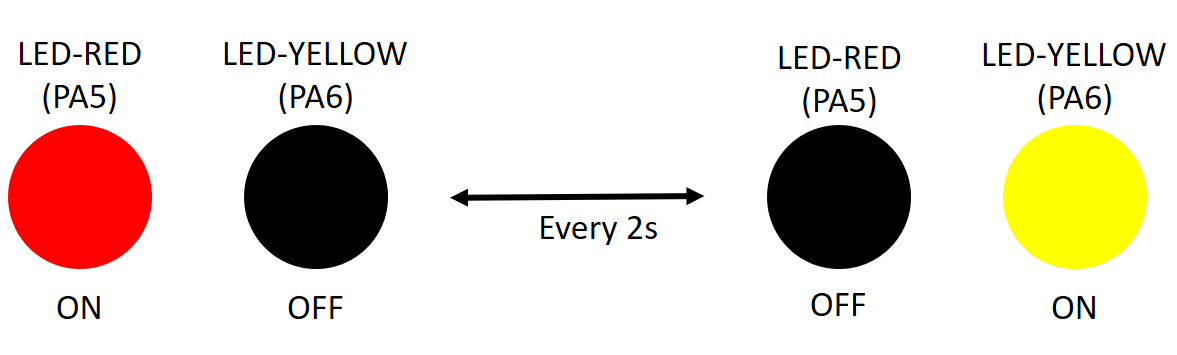
\includegraphics[width=5in]{source/picture/bai_1/pic1.PNG}
    \caption{\textit{State transitions for 2 LEDs}}
    \label{bai1_pic1}
\end{figure}

\textbf{Report 1: }Depict the schematic from Proteus simulation in this report. The caption of the figure is a downloadable link to the Proteus project file (e.g. a github link).\\

\textbf{Report 2: } Present the source code in the infinite loop while of your project. If a user-defined functions is used, it is required to present in this part. A brief description can be added for this function (e.g. using comments). A template to present your source code is presented bellow.

\begin{lstlisting}[caption=An example for your source code]
while (1){
	HAL_GPIO_TogglePin(GPIOA, GPIO_PIN_5);
	HAL_Delay(1000);
}
\end{lstlisting}

\subsection{Exercise 2}
Extend the first exercise to simulate the behavior of a traffic light. A third LED, named \textbf{LED-GREEN} is added to the system, which is connected to \textbf{PA7}. A cycle in this traffic light is 5 seconds for the RED, 2 seconds for the YELLOW and 3 seconds for the GREEN. The LED-GREEN is also controlled by its negative pin.\\

Similarly, the report in this exercise includes the schematic of your circuit and a your source code in the while loop.

\textbf{Report 1: } Present the schematic.\\

\textbf{Report 2: } Present the source code in while.

\subsection{Exercise 3}
Extend to the 4-way traffic light. Arrange 12 LEDs in a nice shape to simulate the behaviors of a traffic light. A reference design can be found in the figure bellow.

\begin{figure}[!htp]
    \centering
    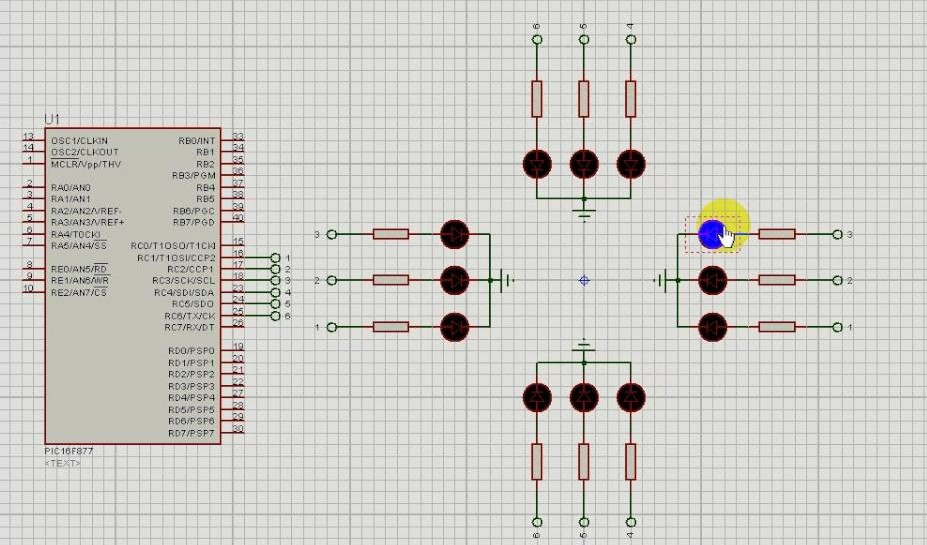
\includegraphics[width=5in]{source/picture/bai_1/pic2.jpg}
    \caption{\textit{Reference design for a 4 way traffic light}}
    \label{bai1_pic2}
\end{figure}

\subsection{Exercise 4}
Add \textbf{only one 7 led segment} to the schematic in Exercise 3. This component can be found in Proteus by the keyword \textbf{7SEG-COM-ANODE}. For this device, the common pin should be connected to the power supply and other pins are supposed to connected to PB0 to PB6. Therefore, to turn-on a segment in this 7SEG, the STM32 pin should be in logic 0 (0V).\\

Implement a function named \textbf{display7SEG(int num)}. The input for this function is from 0 to 9 and the outputs are listed as following:

\begin{figure}[!htp]
    \centering
    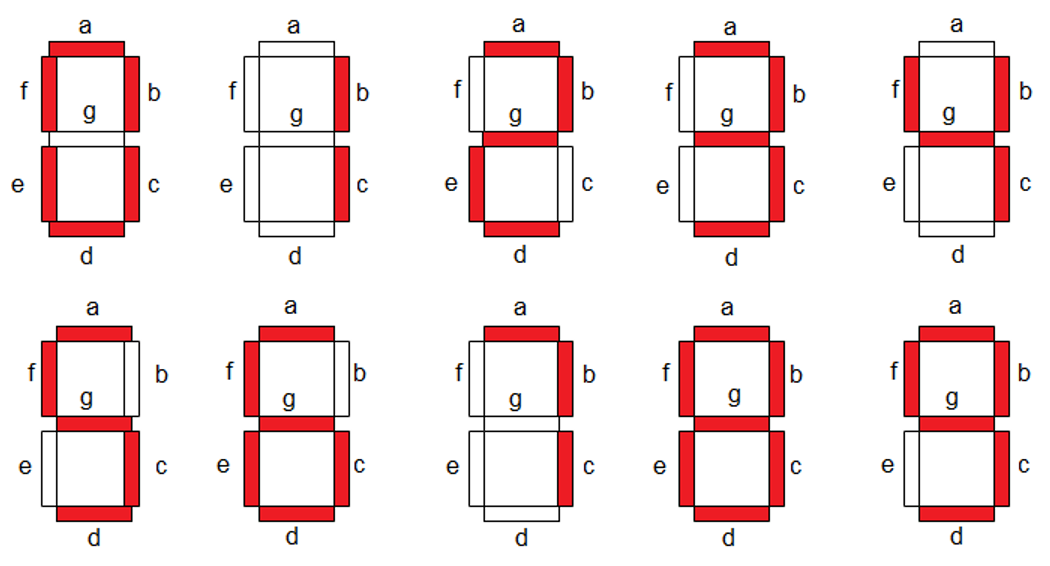
\includegraphics[width=4in]{source/picture/bai_1/pic3.PNG}
    \caption{\textit{Display a number on  7 segment LED}}
    \label{bai1_pic3}
\end{figure}

\newpage
This function is invoked in the while loop for testing as following:
\begin{lstlisting}[caption=An example for your source code]
int counter = 0;
while (1){
    if(counter >= 10) counter = 0;    
    display7SEG(counter++);
    HAL_Delay(1000);

}
\end{lstlisting}

\textbf{Report 1: } Present the schematic.\\

\textbf{Report 2: } Present the source code for display7SEG function.

\subsection{Exercise 5}
Integrate the 7SEG-LED to the 4 way traffic light. In this case, the 7SEG-LED is used to display countdown value.\\

In this exercise, only source code is required to present. The function display7SEG in previous exercise can be re-used.

\subsection{Exercise 6}
In this exercise, a new Proteus schematic is designed to simulate an analog clock, with 12 different number. The connections for 12 LEDs are supposed from PA4 to PA15 of the STM32. The arrangement of 12 LEDs is depicted as follows.

\begin{figure}[!htp]
    \centering
    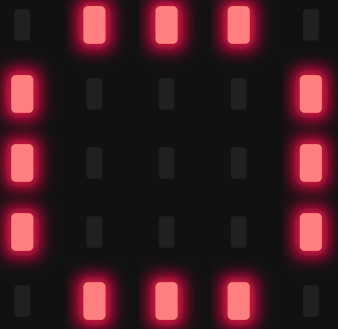
\includegraphics[width=3in]{source/picture/bai_1/pic4.PNG}
    \caption{\textit{12 LEDs for an analog clock}}
    \label{bai1_pic3a}
\end{figure}

Report 1: Present the schematic.
Report 2: Implement a simple program to test the connection of every single LED. This testing program should turn every LED in a sequence.

\subsection{Exercise 7}
Implement a function named \textbf{clearAllClock()} to turn off all 12 LEDs. Present the source code of this function.

\begin{lstlisting}[caption=Function Implementation]
void clearAllClock(){
    //TODO
}
\end{lstlisting}

\subsection{Exercise 8}
Implement a function named \textbf{setNumberOnClock(int num)}. The input for this function is from \textbf{0 to 11} and an appropriate LED is turn on. Present the source code of this function.

\subsection{Exercise 9}
Implement a function named \textbf{clearNumberOnClock(int num)}. The input for this function is from \textbf{0 to 11} and an appropriate LED is turn off. 

\subsection{Exercise 10}
Integrate the whole system and use 12 LEDs to display a clock. At a given time, there are only 3 LEDs are turn on for hour, minute and second information.